\documentclass[a4paper,10pt,twocolumn]{article}
\usepackage[utf8]{inputenc}
\usepackage{graphicx}
\usepackage{setspace}
\usepackage{caption}
\usepackage{amsmath}
\usepackage{listings}


%\lstset{language=Python}
%\lstset{frame=lines}
%\lstset{caption={Insert code directly in your document}}
%\lstset{label={lst:code_direct}}
%\lstset{basicstyle=\footnotesize}


\setstretch{1.2}

%opening
\title{Embeded silicon crystals: Calculating properties from Raman Spectra}
\author{Antony Lopez Sánchez, Giovanni Eboli Castro, \\ Daniel Carlos Palacios Hernandez, David Omar Flores Tavira}

\begin{document}

\twocolumn[
  \begin{@twocolumnfalse}
    \maketitle
    \begin{abstract}
    In the present document we explore the characterization by means of Raman spectroscopy of a quartz matrix with embeded silicon nano crystals (Si-NC) A total of 20 Raman spectrums (RS) where taken along the widest axis of the sample. The RS  shown a change in shape of the LO and TO transitions due to a change in the crystal size (according to the literature and the observations discussed in this document). The analysis of the RS where made using a python script available online to later implementations. Using the  algorithm a multi peak signal was fited to the observations.
    \end{abstract}
    \vspace{1cm}
  \end{@twocolumnfalse}
]

\section{Introduction}

Silicon is an indirect band gap semiconductor $ (~1.1 \quad eV) $ with a high refractive index and low light absorption in the visible spectrum. It is transparent to infrared radiation, which makes it useful in optics and solar cell technologies. Crystalline silicon has a diamond-like crystal structure, known as a diamond cubic structure, the lattice constant is approximately 0.5431 nm.

Silicon nanocrystals, also known as silicon quantum dots, possess unique properties at the nanoscale that make them useful in a variety of applications like: optoelectronics, where silicon nanocrystals can emit light in the visible and near-infrared range due to their quantum confinement effect; bioimaging and bioengineering, their small size, chemical stability, and tunable emission wavelengths make them ideal for labeling and tracking biological entities.

It is possible to identify the silicon crystal structure analyzing its Raman spectrum, the conservation of phonon momentum q in crystalline silicon leaves as Raman active mode only the zone center $(q=0) $ optical phonon at, which produces a single peak of high intensity. In the other hand, amorphous silicon exhibits a q-selection rule relaxation due to the loss in long range order, which produces broadening on the silicon main peak and shifting towards lower wave numbers.

\begin{figure}
  \centering
  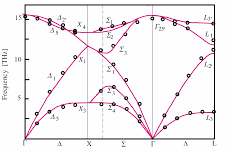
\includegraphics[scale=0.9]{relacionesdedispersiondefonones.png}
  \captionof{figure}{Silicon phonon dispersion diagram.} % Add captn 2 the f
\end{figure}

To create silicon nanocrystals using sputtering, a silicon target is typically bombarded with inert gas ions, such as argon (Ar). The high-energy ion bombardment causes silicon atoms to be dislodged from the target surface. These silicon atoms then condense and nucleate on the substrate, forming nanocrystals. Various parameters can be controlled during the sputtering process to influence the growth of silicon nanocrystals. These parameters include sputtering power, sputtering gas pressure, substrate temperature, and deposition time. By adjusting these parameters, researchers can tailor the size, density, and distribution of silicon nanocrystals in the thin film.


\section{Experimental Details}
The sample in which the analysis was carried on is a quartz matrix with embeded silicon nanocrystals processed by Sputtering RF, with the density of the crystals varying along the sample. A High Resolution Raman Spectrometer was used in this experiment (LabRam HR600) with an excitation wavelenght
of 633nm, Acquisition time of 10 seconds, 2 accumulations, wavenumber (in $cm^{-1}$ ) between (100,1000) and the Hole at 75\%. The spectrums where taken with a separation in the x axis of 140$\mu m$

\begin{figure}[h]
  \centering
  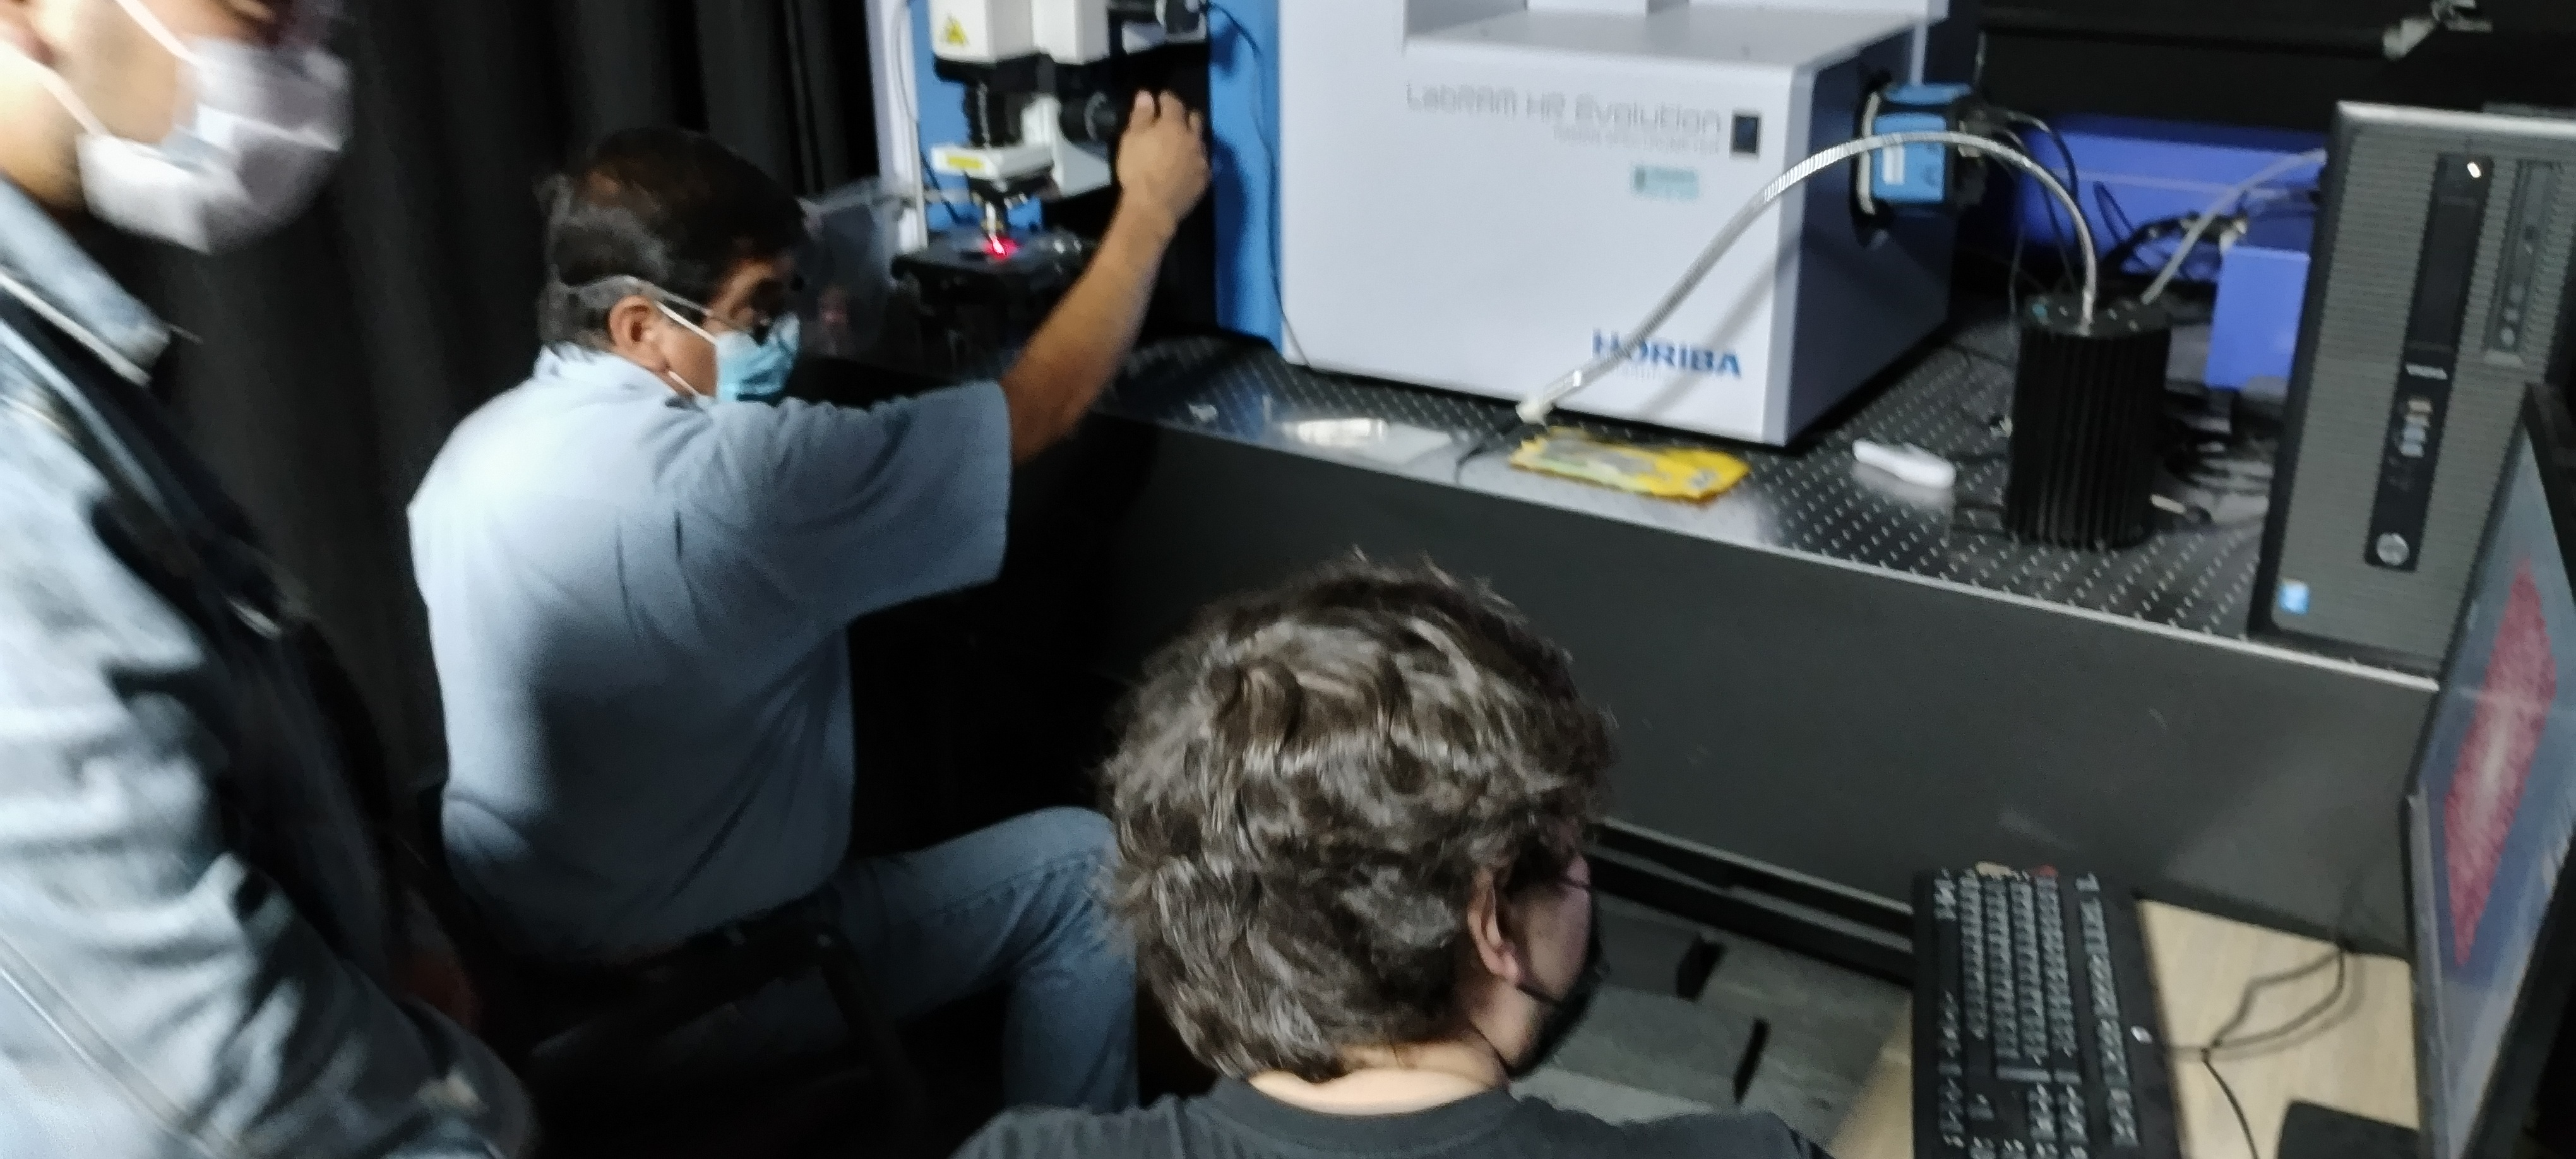
\includegraphics[scale=.055]{raman.jpg}
  \captionof{figure}{Manipulation of the Rama Spectrometer to focus the excitation source on the surface of the sample} % Add captn 2 the f
\end{figure}


\begin{figure}[h]
  \centering
  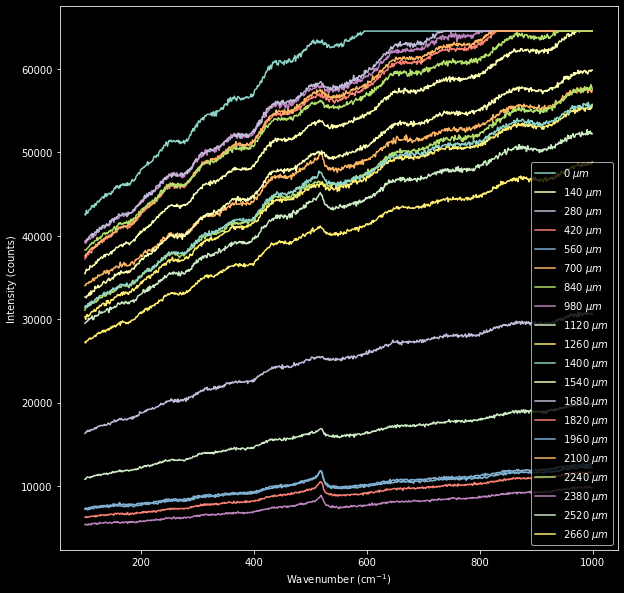
\includegraphics[height=8cm, width=7cm]{all_n.png}
  \captionof{figure}{Raman spectrums for the sample taken at different x positions.} % Add captn 2 the f
\end{figure}


The RS are shown in Figure 3. All the signals present a baseline that is aparentally a linearly increasing emission in all the wavenumbers. We observe an increase of the slope in the RS as the measurements are made in different points along the sample. To start the analysis we pick a range of wavenumber between 350 cm$^{-1}$ and 600 cm$^{-1}$ this is because we can expect the region of interest between the si transition at 520 $cm^{-1}]$ and the region in which the transitions start to occur in the RS (400 $cm^{-1}$). Then we can substract the baseline as shown in Figure 4.

\begin{figure}[h]
  \centering
  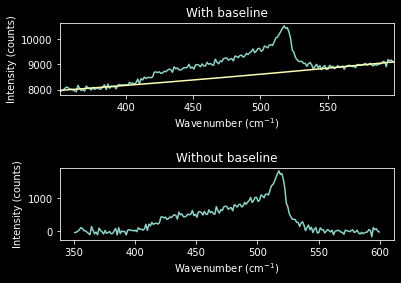
\includegraphics[width=0.9\columnwidth, height=4cm]{baseline.png}
  \captionof{figure}{Raman Spectrum before and after doing the base line correction, in the software we fit a polinomial of degree 3 but it can be changed.} % Add captn 2 the f
\end{figure}

The calculation for the baseline is made using a polinomial fit and it can be tweaked according to specific cases:


\lstset{caption={Example code to crop a region and calculate baseline}}
\begin{lstlisting}[basicstyle=\fontsize{5}{4}\selectfont\ttfamily]
# Code to crop a region of interest
# and calculate a baseline

import numpy as np

# Accessing to the x and y points of the RS
spectrum = RamanSpectrum('medicion_silicio.txt')
x,y = spectrum.x, spectrum.y

def crop(upper,lower,X,Y):
    x_c = []
    y_c = []
    for a,b in zip(X,Y):
        if lower < a < upper:
            x_c.append(a)
            y_c.append(b)
    # We return the cropped range
    return x_c, y_c;

# We store the cropped values inside
# new arrays x_n and y_n

x_n, y_n = crop(600,300,x,y)

# X and Y are arrays that store the
# coordinates of the RS, in this
# function we calculate a baseline
# for the pair of x,y, which x satisfies
# (x < x_1),( x_2 < x) with ( x_1 < x_2).

def fit_baseline(x_1,x_2,X,Y, ord):
    x_f =[]
    y_f =[]
    for a,b in zip(X,Y):
        if (x<x_1) and (x_2<x):
            x_f.append(a)
            y_f.append(b)
    baseline = np.polyfit(x_f,y_f,ord)
    return baseline;

\end{lstlisting}

After this we can start to fit the signal to a sum of three gaussian curves, this are defined by the equation 1:

\begin{equation}
f(x) = \frac{1}{\sigma \sqrt{2\pi}} e^{-\frac{(x - \mu)^2}{2\sigma^2}}
\end{equation}

In the last equation the factor that is multipliyng the exponential is the amplitute of the gaussian and  $\mu$ is the value at which the gaussian is centered, if we consider that our signal is generated by the sum of three gaussian curves and the amplitute of each one is $A_{n}$ with a center $\mu_{n}$ the analytical function to fit writes as follows:

\begin{equation}
f(x) = \sum_{n = 1}^{3} A_{n} e^{-\frac{(x - \mu_{n})^2}{2\sigma^2}}
\end{equation}

With a python package we can define the function to be optimized, and a fitting function can be defined setting a number of peaks to adjust (in our case 3 peaks) by least squares.

\lstset{caption={Multipeak fitting of three gaussian curves}}
\begin{lstlisting}[basicstyle=\fontsize{5}{4}\selectfont\ttfamily]

# Importing the optimization function

from scipy.optimize import curve_fit
import numpy as np

# Define the gaussian generator

def gaussian( x, amplitude, center, sigma):
    return amplitude * np.exp(-(x - center)**2 / (2 * sigma**2))

# The multi peak function

def multi_peak_fit( x, *params):
    num_peaks = len(params) // 3
    y_fit = np.zeros_like(x)

    for i in range(num_peaks):
        amplitude, center, sigma = params[i*3 : (i+1)*3]
        y_fit += gaussian(x, amplitude, center, sigma)
    return y_fit;

# Creating the initial parameters to fit
# this parameters may change.
# the format to fill this parameters is due
# to the construction of the function
# which is amplitude, center and sigma

params = [1000, 515, 20]
params.append(500,500,40)
params.append(100,480,60)

popt, pcov = curve_fit(multi_peak_fit, x, y, p0=params)

\end{lstlisting}

\section{Results and discussion}
The training process of GPT involves pre-training on large corpora and subsequent fine-tuning on specific downstream tasks. We describe the pre-training phase, which involves predicting masked tokens in a language modeling objective. We discuss the challenges and considerations in training GPT on massive datasets, as well as techniques to enhance its performance and efficiency. Furthermore, we delve into the fine-tuning process, where GPT is adapted to specific tasks through supervised learning.

    \begin{equation}
    \int_{a}^{b}
    \end{equation}

\section{Applications of GPT}
GPT has demonstrated remarkable versatility across a wide array of NLP applications. We provide an overview of the various tasks where GPT has excelled, such as language translation, text summarization, question answering, and sentiment analysis. For each task, we discuss the methodologies employed and the corresponding performance of GPT. We also examine the ethical implications and potential biases that arise when using GPT in real-world applications.

\section{Strengths and Limitations}
While GPT has achieved impressive results, it also exhibits certain limitations. We analyze the strengths and weaknesses of GPT in different contexts, including long-range dependency modeling, handling rare or out-of-distribution words, and dealing with biased or harmful content. We highlight the challenges that researchers and practitioners face when working with GPT and propose potential avenues for improvement.

\section{Conclusion}
In this paper, we have presented a comprehensive analysis of GPT, examining its architecture, training process, and applications. GPT has significantly advanced the field of NLP, demonstrating its capabilities in generating coherent and contextually appropriate text. However, challenges remain in mitigating biases, improving long-range dependency modeling, and addressing ethical concerns. As the field progresses, further research and innovation will pave the way for the continued advancement and responsible use of GPT in diverse real-world applications.
\section{References}
\small{
[1]\textsc{Narasimha Rao Mavilla,  Chetan Singh Solanki ,  Juzer Vasi} \\
\textit{Raman spectroscopy of silicon nanocrystals fabricated by inductively coupled plasma chemical vapor deposition}\\
    Volume 52, August 2013, Pages 59-64 \\
https://doi.org/10.1016/j.physe.2013.03.019 \\

    [2]\textsc{Katerina V. Michailovska, Ivan Z. Indutnyi, Petro E. Shepeliavyi, Mykola V. Sopinskyy, Viktor A. Dan’ko, Zinoviia F. Tsybrii, Andrii S. Nikolenko} \\
\textit{Samarium‑induced enhancement of $ SiO_{x} $ decomposition and Si nanocrystals formation. }
Applied Nanoscience \\
    https://doi.org/10.1007/s13204-022-02617-0 \\

    [3]\textsc{H. Richter, Z.P. Wang , and L. Ley}\\
\textit{The phonon Raman spetrum in microcrystaline silicon }
Applied Nanoscience \\
    Max-Planck-Institut fiir FestkBrperforschung, Heisenbergstr. 1, 7000 Stuttgart 80, Federal Republic of Germany

    [4]\textsc{Guadalupe Monroy Rodríguez} \\
\textit{Caracterización óptica de películas de silicio y SiO2 crecidas por las técnicas de Erosión Catódica (sputtering) y Ablación Láser } \\
Tesis de maestría ESFM-IPN \\

    [5]\textsc{Cedrik Meier,  Stephan Lüttjohann,  Vasyl G. Kravets}\\
\textit{Raman properties of silicon nanoparticles}\\
    Volume 32, Issues 1–2, May 2006, Pages 155-158 \\
    https://doi.org/10.1016/j.physe.2005.12.030 \\
}

\end{document}
